
%package list
\documentclass{article}
\usepackage{amsmath}
\usepackage[top=3cm, bottom=3cm, outer=3cm, inner=3cm]{geometry}
\usepackage{multicol}
\usepackage{graphicx}
\usepackage{url}
%\usepackage{cite}
\usepackage{hyperref}
\usepackage{array}
%\usepackage{multicol}
\newcolumntype{x}[1]{>{\centering\arraybackslash\hspace{0pt}}p{#1}}
\usepackage{natbib}
\usepackage{pdfpages}
\usepackage{multirow}
\usepackage[normalem]{ulem}
\useunder{\uline}{\ul}{}
\usepackage{svg}
\usepackage{xcolor}
\usepackage{listings}
\lstdefinestyle{ascii-tree}{
    literate={├}{|}1 {─}{--}1 {└}{+}1 
  }
\lstset{basicstyle=\ttfamily,
  showstringspaces=false,
  commentstyle=\color{red},
  keywordstyle=\color{blue}
}
%\usepackage{booktabs}
\usepackage{caption}
\usepackage{subcaption}
\usepackage{float}
\usepackage{array}

\newcolumntype{M}[1]{>{\centering\arraybackslash}m{#1}}
\newcolumntype{N}{@{}m{0pt}@{}}


%%%%%%%%%%%%%%%%%%%%%%%%%%%%%%%%%%%%%%%%%%%%%%%%%%%%%%%%%%%%%%%%%%%%%%%%%%%%
%%%%%%%%%%%%%%%%%%%%%%%%%%%%%%%%%%%%%%%%%%%%%%%%%%%%%%%%%%%%%%%%%%%%%%%%%%%%
\newcommand{\itemEmail}{ccapatinta@unsa.edu.pe}
\newcommand{\itemStudent}{Capatinta Almanza Camilo B. A.}
\newcommand{\itemCourse}{Análisis y Diseño de Algoritmos}
\newcommand{\itemCourseCode}{1702231}
\newcommand{\itemSemester}{IV}
\newcommand{\itemUniversity}{Universidad Nacional de San Agustín de Arequipa}
\newcommand{\itemFaculty}{Facultad de Ingeniería de Producción y Servicios}
\newcommand{\itemDepartment}{Departamento Académico de Ingeniería de Sistemas e Informática}
\newcommand{\itemSchool}{Escuela Profesional de Ingeniería de Sistemas}
\newcommand{\itemAcademic}{2026 - B}
\newcommand{\itemInput}{Del 03 septiembre 2026}
\newcommand{\itemOutput}{Al 09 septiembre 2026}
\newcommand{\itemPracticeNumber}{01}
\newcommand{\itemTheme}{M.C.D. y Algoritmo de Euclides}
%%%%%%%%%%%%%%%%%%%%%%%%%%%%%%%%%%%%%%%%%%%%%%%%%%%%%%%%%%%%%%%%%%%%%%%%%%%%
%%%%%%%%%%%%%%%%%%%%%%%%%%%%%%%%%%%%%%%%%%%%%%%%%%%%%%%%%%%%%%%%%%%%%%%%%%%%

\usepackage[english,spanish]{babel}
\usepackage[utf8]{inputenc}
\AtBeginDocument{\selectlanguage{spanish}}
\renewcommand{\figurename}{Figura}
\renewcommand{\refname}{Referencias}
\renewcommand{\tablename}{Tabla} %esto no funciona cuando se usa babel
\AtBeginDocument{%
	\renewcommand\tablename{Tabla}
}

\usepackage{fancyhdr}
\pagestyle{fancy}
\fancyhf{}
\setlength{\headheight}{40.51407pt}
\renewcommand{\headrulewidth}{1pt}
\renewcommand{\footrulewidth}{1pt}
\fancyhead[L]{\raisebox{-0.2\height}{
\includegraphics[width=3cm]{img/logo_episunsa.png}}}
\fancyhead[C]{\fontsize{7}{7}\selectfont	\itemUniversity \\ \itemFaculty \\ \itemDepartment \\ \itemSchool \\ \textbf{\itemCourse}}
\fancyhead[R]{\raisebox{-0.2\height}{
\includegraphics[width=1.2cm]{img/logo_abet}}}
\fancyfoot[L]{Estudiante Capatinta Camilo}
\fancyfoot[C]{\itemCourse}
\fancyfoot[R]{Página \thepage}

% para el codigo fuente
\usepackage{listings}
\usepackage{color, colortbl}
\definecolor{dkgreen}{rgb}{0,0.6,0}
\definecolor{gray}{rgb}{0.5,0.5,0.5}
\definecolor{mauve}{rgb}{0.58,0,0.82}
\definecolor{codebackground}{rgb}{0.95, 0.95, 0.92}
\definecolor{tablebackground}{rgb}{0.8, 0, 0}

\lstset{frame=tb,
	language=bash,
	aboveskip=3mm,
	belowskip=3mm,
	showstringspaces=false,
	columns=flexible,
	basicstyle={\small\ttfamily},
	numbers=none,
	numberstyle=\tiny\color{gray},
	keywordstyle=\color{blue},
	commentstyle=\color{dkgreen},
	stringstyle=\color{mauve},
	breaklines=true,
	breakatwhitespace=true,
	tabsize=3,
	backgroundcolor= \color{codebackground},
}

\begin{document}
	
	\vspace*{10px}
	
	\begin{center}	
		\fontsize{17}{17} \textbf{ Actividad \itemPracticeNumber}
	\end{center}
	\centerline{\textbf{\Large Tema: \itemTheme}}
	%\vspace*{0.5cm}	

	\begin{flushright}
		\begin{tabular}{|M{2.5cm}|N|}
			\hline 
			\rowcolor{tablebackground}
			\color{white} \textbf{Nota}  \\
			\hline 
			     \\[30pt]
			\hline 			
		\end{tabular}
	\end{flushright}	

	\begin{table}[h!]
		\begin{tabular}{|x{4.7cm}|x{4.8cm}|x{4.8cm}|}        
			\hline 
			\rowcolor{tablebackground}
			\color{white} \textbf{Estudiante} & \color{white}\textbf{Escuela}  & \color{white}\textbf{Asignatura}   \\
			\hline 
			{\itemStudent \par \itemEmail} & \itemSchool & {\itemCourse \par Semestre: \itemSemester \par Código: \itemCourseCode}     \\
			\hline 			
		\end{tabular}
	\end{table}		
	
	\begin{table}[H]
		\begin{tabular}{|x{4.7cm}|x{4.8cm}|x{4.8cm}|}
			\hline 
			\rowcolor{tablebackground}
			\color{white}\textbf{Actividad} & \color{white}\textbf{Tema}  & \color{white}\textbf{Duración}   \\
			\hline 
			\itemPracticeNumber & \itemTheme & 04 horas   \\
			\hline 
		\end{tabular}
	\end{table}
	
	\begin{table}[H]
		\begin{tabular}{|x{4.7cm}|x{4.8cm}|x{4.8cm}|}
			\hline 
			\rowcolor{tablebackground}
			\color{white}\textbf{Semestre académico} & \color{white}\textbf{Fecha de inicio}  & \color{white}\textbf{Fecha de entrega}   \\
			\hline 
			\itemAcademic & \itemInput &  \itemOutput  \\
			\hline 
		\end{tabular}
	\end{table}
	
	\section{Tarea de Investigación}
	\begin{itemize}		
		\item ¿Qué es y cómo funciona el Máximo Común Divisor?
		\item ¿Qué es y cómo funciona el Algoritmo de Euclides?
		\item Proponga una solución distinta (C++).
	\end{itemize}
		
	\section{Resolución de actividades}
	
	\subsection{¿Qué es y cómo funciona el Máximo Común Divisor?}

    El Máximo Común Divisor (MCD) de dos números enteros es el número más grande que divide exactamente a ambos sin dejar residuo. Por ejemplo, 
    para los números 8 y 12, los factores comunes son 1, 2 y 4. Como este último es el factor más grande, entonces se dice que el
    MCD de 8 y 12 es 4 (MCD(8,12)=4).


	\subsection{¿Qué es y cómo funciona el Algoritmo de Euclides?}

    El algoritmo de Euclides es un método eficiente para calcular el máximo común divisor de dos números enteros. Lleva el nombre del antiguo matemático griego Euclides, quien lo describió por primera vez en Elementos (ca. 300 a. C.). El algoritmo euclidiano se basa en el principio de que el máximo común divisor de dos números no cambia si el número más grande se reemplaza por su diferencia con el número más pequeño. Es un método para encontrar el MCD mediante la división repetida y el uso del residuo. El proceso se repite hasta que uno de los números se convierte en cero, el otro número es el MCD.
		
    \begin{align*}
    48 \bmod 18 &= 12 \\
    18 \bmod 12 &= 6 \\
    12 \bmod 6 &= 0 \quad \Rightarrow \quad \text{MCD} = 6
    \end{align*}
	
	\subsection{Solución alternativa en C++}

	%\begin{itemize}	
	%	\item Se creo el archivo \textbf{.gitignore} para no considerar los archivos %\textbf{*.class} que son innecesarios hacer seguimiento.
	%\end{itemize}
	%\begin{lstlisting}[language=bash,caption={Creando .gitignore}]
	%	$ vim lab01/.gitignore
	%\end{lstlisting}
	%\begin{lstlisting}[language=bash,caption={lab01/.gitignore}]
	%	*.class
	%\end{lstlisting}
	%\begin{lstlisting}[language=bash,caption={Commit: Creando .gitignore para archivos *.class}]
	%	$ git add .
	%	$ git commit -m "Creando .gitignore para archivos *.class"			
	%	$ git push -u origin main
	%\end{lstlisting}
	
	\clearpage
	
	%\begin{lstlisting}[language=bash,caption={Creando .gitignore}]
	%	$ vim lab01/Insertion.java
	%\end{lstlisting}
	
	\lstinputlisting[language=c++, caption={Solución alternativa en C++},numbers=left,]{src/newAlgotihm.cpp}

    \begin{itemize}
        \item En el código anterior se puede observar el código de la solución alternativa.
        \item De la línea 7 - 21 se implementa la solucion propuesta. 
        \item En la línea 24 - 27 se implementa la solución de Euclides. 
        \item En main() se hace la comparación de ambos algoritmos, dejando en evidencia que Euclides es por mucho más eficiente. 
    \end{itemize}

    \begin{figure}[H]
    \centering
    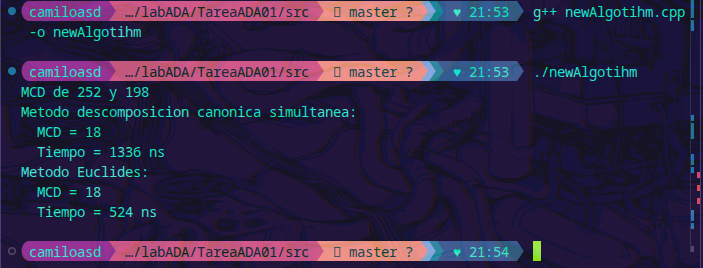
\includegraphics[width=0.8\textwidth]{img/runAlgotihm.png}
    \caption{Algoritmo propuesto en comparación con Euclides}
    \label{fig:diagrama}
    \end{figure}
    
\section{Referencias}
\begin{itemize}
    \item Wikipedia. (2025). \textit{Máximo común divisor}. Recuperado de \url{https://es.wikipedia.org/wiki/M\%C3\%A1ximo_com\%C3\%BAn_divisor}
    \item Wikipedia. (2025). \textit{Algoritmo de Euclides}. Recuperado de \url{https://es.wikipedia.org/wiki/Algoritmo_de_Euclides}
    \item Informatec Digital. (2025). \textit{El Algoritmo de Euclides: Historia, Uso y Aplicaciones}. Recuperado de \url{https://informatecdigital.com/el-algoritmo-de-euclides/}
\end{itemize}
	
%\clearpage
%\bibliographystyle{apalike}
%\bibliographystyle{IEEEtranN}
%\bibliography{bibliography}
			
\end{document}